\label{sec:hadronictrigger}
Triggers suitable for hadronic SUSY searches at the LHC typically manage to suppress the overwhelming QCD background by requiring events to have a large $\met$ as a criterion for firing the trigger. Additionally, a minimum amount of $\Ht$ can also be required, or, for that matter, some combination of $\met$ and $\Ht$. However, because   online calculations of observables must be extremely rapid, only rough approximations of the $\Ht$ and $\met$ can be obtained in real time. Substantial discrepancies can arise between the more approximate online objects and the more precise offline objects, the latter enjoying increased availability of time and computing resources, and can afford to be much more precise. In order to guarantee that a trigger fire on events with at least a given amount of $\met$, the trigger threshold on the online $\met$ must be sufficiently lower than the offline value ensure a 100\% probability that an event in the signal region would actually have been accepted by the trigger. This introduces the concept of a trigger turn-on curve, which is a monicker for a plot of the probability (efficiency) of a trigger to select an event as a function of an offline variable. $\met$ trigger turn-on curves have notoriously gradual slopes, since the calculation of the $\met$ is particularly sensitive to jet energy resolutions, which differ substantially in the offline and online event reconstruction.

There are two conditions that must be met in order for a trigger to be useful. First, it must have a sufficiently high efficiency for selecting signal events. And second, it must be possible to make an unbiased measurement of the trigger efficiency. The latter can be a non-trivial task, since in order to measure the efficiency without bias, one needs a sample of events, referred to as a reference sample, that is independent of the events that pass the trigger. Concretely, suppose the goal is to make a measurement of the efficiency of trigger A. One can make an unbiased measurement by obtaining a sample of events collected by trigger B, so long as the absolute probability of firing trigger A, P(A), is equal to the conditional probability of trigger A firing given that trigger B has also fired, P(A$|$B):
\begin{equation}
\text{P(A)} = \text{P(A|B)}.
\label{eq:trigcondition}
\end{equation}
In other words, trigger B should be chosen such that its triggering criteria are independent of those of trigger A. Whether or not Equation \ref{eq:trigcondition} holds can be verified in simulation. Finally, the unbiased estimate of the efficiency of trigger A is the fraction of events that fire trigger B that also fire trigger A:
\begin{equation}
\hat{\epsilon}_{\text{A}} = \frac{N_{\text{fire A and B}}}{N_{\text{fire B}}}.
\label{eq:trigeff}
\end{equation}
This is an estimate of P(A|B), with an expectation value equal to P(A) if, and only if, P(AB) = P(A)P(B), that is triggers A and B are independent.

In the case of the 2015 hadronic SUSY analyses, data were collected by a trigger named
\begin{itemize}
  \item \texttt{HLT\_PFHT350\_PFMET100\_*},
\end{itemize}
referred to as the primary trigger (trigger A). Here, PFHT and PFMET refer to the online $\Ht$ and $\met$ computed using the particle flow algorithm, and the numbers 350 and 100 refer to the respective triggering thresholds in units of GeV. The asterisk indicates that, for technical reasons, different versions of this trigger were used at different stages of data taking. I estimated the trigger efficiency as a function of the offline $\Ht$
and $\mht$, following the guidelines outlined for the example of trigger A above. 

I choose trigger B (the reference trigger) to be the trigger named
\begin{itemize}
  \item \texttt{HLT\_Ele27\_eta2p1\_WPLoose\_Gsf\_v*}, 
\end{itemize}
which selects events that contain a reconstructed electron with a $\pt$ greater than 27 GeV,
and take the base sample to be the subset of these events that have $\text{N}_{\text{jets}}>3$ and a single offline reconstructed electron.  A sample of simulated t$\bar{\text{t}}$ events is used to establish the validity of Equation \ref{eq:trigcondition}. First, the conditional probability of firing the primary trigger, given that the reference trigger fired, is computed as a function of the offline $\Ht$ and $\mht$. Then, the absolute probability of firing the primary trigger is computed by replacing the reference sample with the entire sample of simulated events, as a function of the same variables. The ratio of the conditional probability (``method'') to the absolute probability (``truth'') is shown in Fig. \ref{fig:2dEffRatio}. 
\begin{figure}[h]
  \begin{center}
    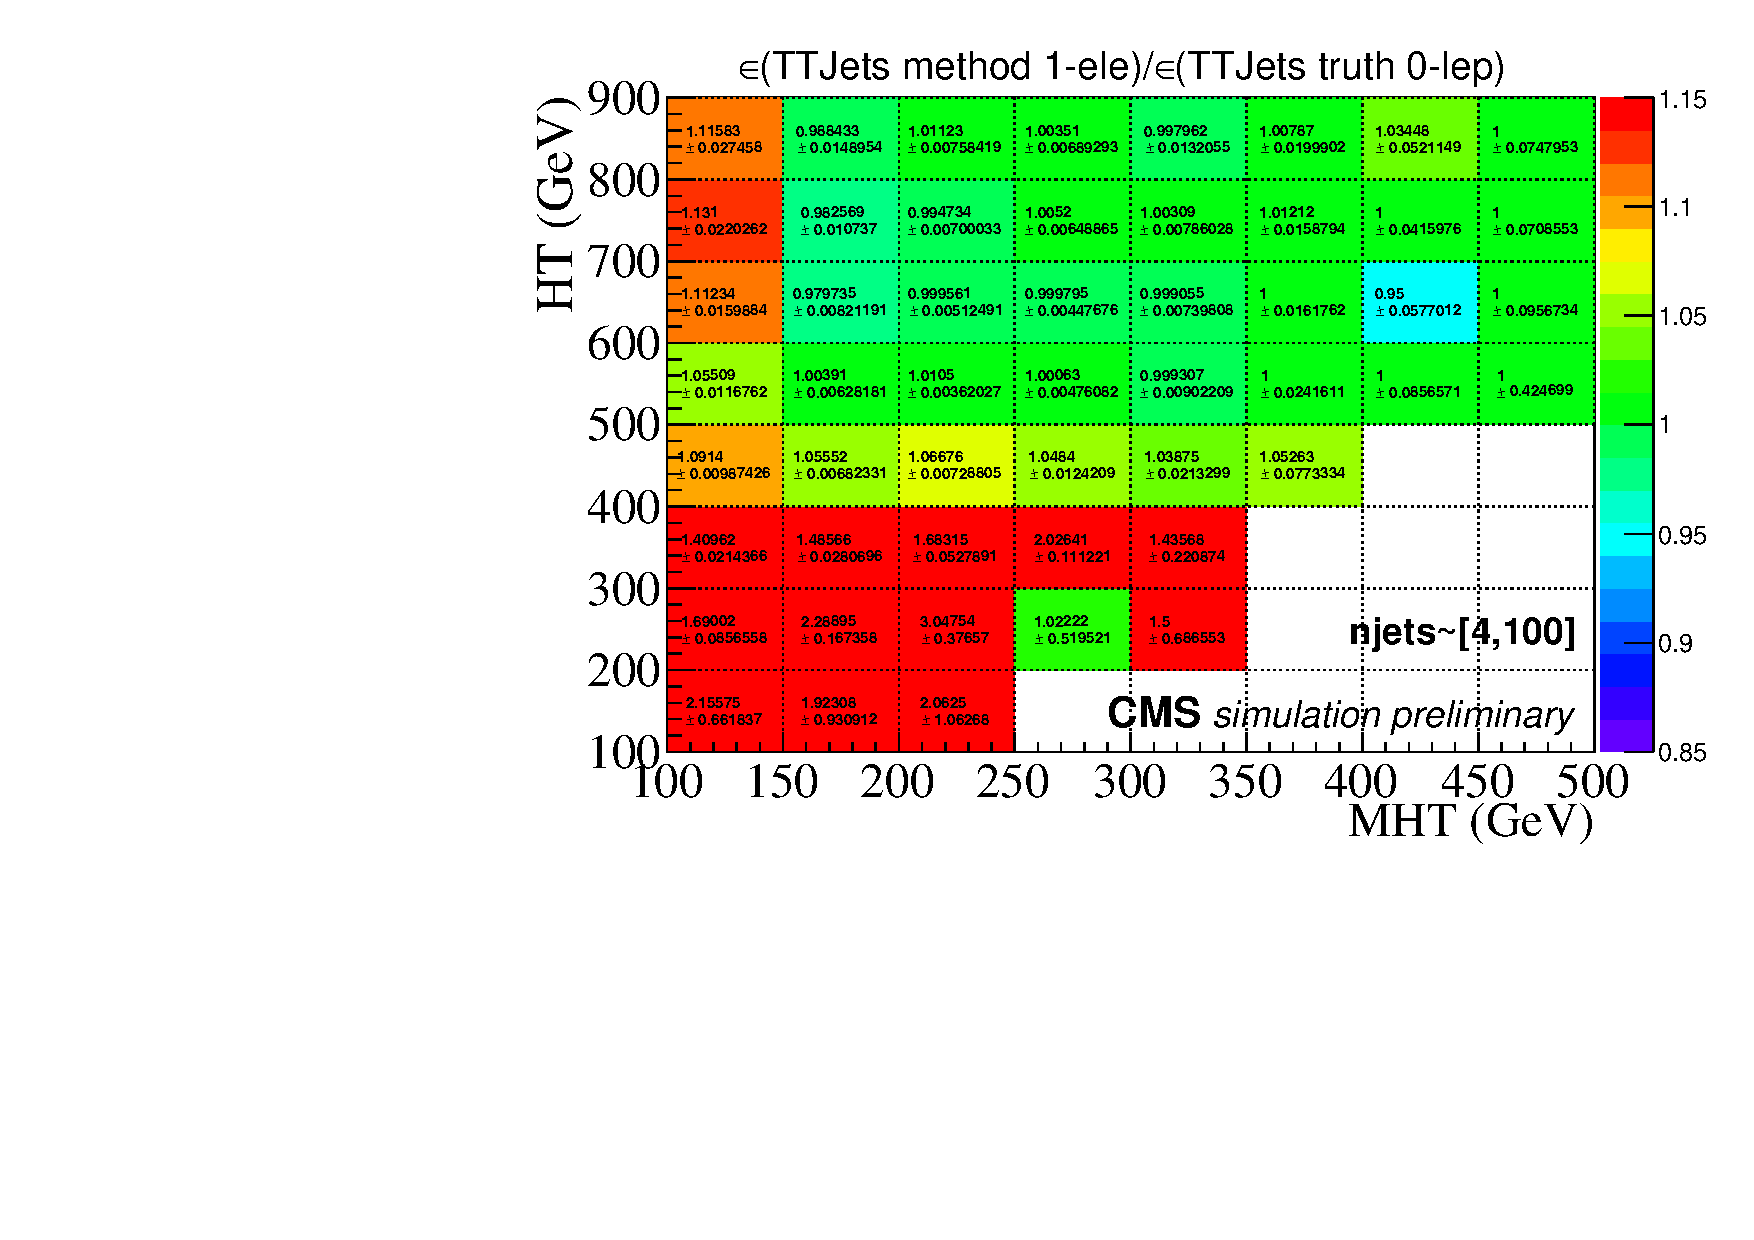
\includegraphics[width=0.95\linewidth]{figures/trigger/EfficiencyRatioMethodTruth.pdf}
    \caption{
      The ratio of the trigger efficiency for events passing the single
      electron reference trigger to the trigger efficiency for all
      events in a simulated $\ttbar$ sample, as a function of the offline $\Ht$
      and $\mht$. The ratio is consistent with 1 within the region of
      the baseline selection of $\Ht>500$ GeV and $\mht>200$ GeV of the CMS hadronic searches.
    }
    \label{fig:2dEffRatio}
  \end{center}
\end{figure}
It is seen that this method, namely, the choice of reference trigger, allows for an unbiased estimate of the trigger efficiency in the region $\mht>150$ GeV and $\Ht>500$, which fortunately includes the baseline selection of the analyses that used this trigger, which impose offline selections of $\mht>200$ GeV and $\Ht>500$ GeV or similar.
These searches, including the multi-jet + $\mht$ search~\cite{Khachatryan:2016kdk}, are briefly summarized in Section \ref{sec:2015results}). 

The efficiency, estimated without bias using Equation \ref{eq:trigeff}, is shown as a function of the offline $\Ht$ and $\mht$, each in 1-dimension, in Fig. \ref{fig:trigger-turnon} using the entire 2015 dataset. 
\begin{figure}[tbp]
  \begin{center}
    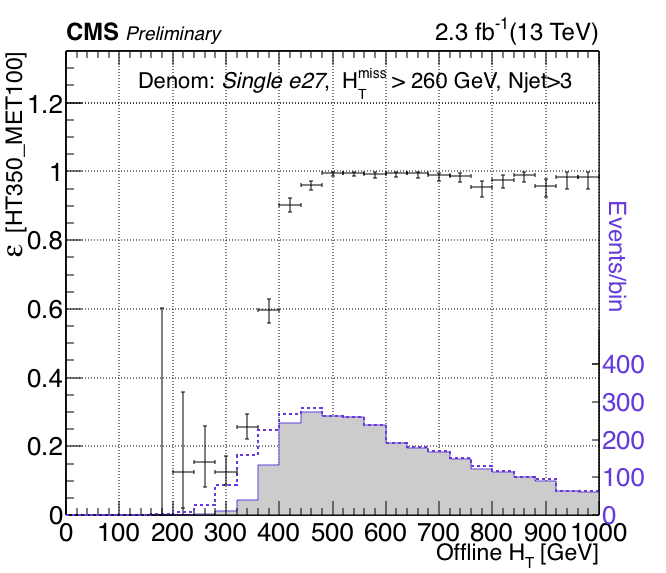
\includegraphics[width=0.49\linewidth]{figures/trigger/EffVsHt2_3InvFb.png}
    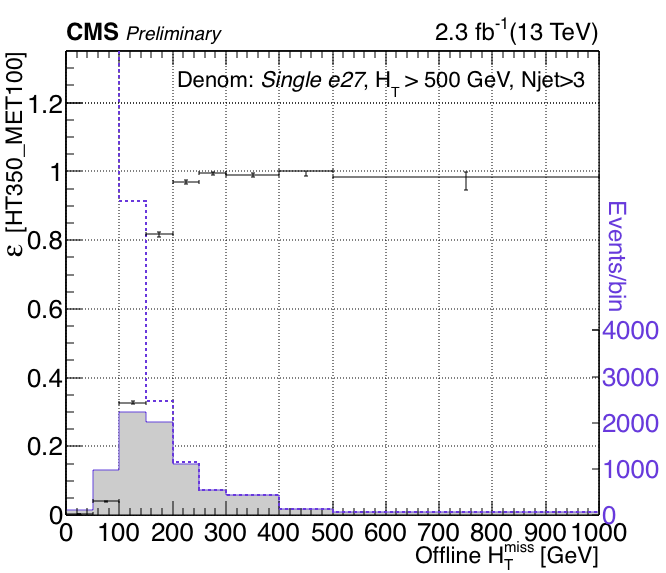
\includegraphics[width=0.49\linewidth]{figures/trigger/EffVsMht2_3InvFb.png}
    \caption{
      The trigger efficiency for \texttt{HLT\_PFHT350\_PFMET100*} 
      as a function of the search variables $\Ht$ and $\mht$. The dashed (solid) blue
      lines show the distributions of the denominator (numerator) samples. These results were used in the CMS PAS on the commissioning of 13 TeV observables for SUSY searches~\cite{CMS-DP-2015-035}.
      }
    \label{fig:trigger-turnon}
  \end{center}
\end{figure}
The statistical uncertainties in the plot are the 68\% CL Clopper-Pearson
intervals~\cite{Clopper:Pearson}. Additionally, a systematic uncertainty is assigned to the efficiency
equal to the difference between the efficiency obtained from applying the method described to a
sample of simulated $\ttbar$ events and that derived
from a set of simulated signal events. Such differences may arise due to any number of subtle differences in the content of the events in $\ttbar$ and signal samples. These uncertainties can be reduced or eliminated by more intelligently choosing a set of observables on which the efficiency estimation depends, in this case the $\Ht$ and $\mht$. This is discussed below under the subsection heading ``Multivariate trigger techniques,'' in the context of more advanced techniques for determining the trigger efficiency. 
\FloatBarrier

\subsubsection{A better trigger: monojet trigger}
There is little reason that the trigger named
\begin{itemize}
  \item \texttt{HLT\_PFMETNoMu90\_PFMHTNoMu90\_*},
\end{itemize}
referred to as the monojet trigger,
was not used in the 2015 multi-jet search. This trigger has no $\Ht$ requirement, and has a lower $\mht$ threshold than that required by the primary trigger. Therefore, the monojet trigger has a higher efficiency in all regions of kinematic phase space, including regions with low $\Ht$ and $\mht$. Furthermore, it is found that, whereas the efficiency estimate for the primary trigger features significant bias in the low $\Ht$ and low $\mht$ regions, indicated by the red portions of the $\Ht-\mht$ plane in Fig. \ref{fig:2dEffRatio}, the equivalent ratio plot for the monojet trigger shows consistency with 1 throughout the entire plane, as seen in Fig. \ref{fig:2dMonoEffRatio}.
\begin{figure}[h]
  \begin{center}
    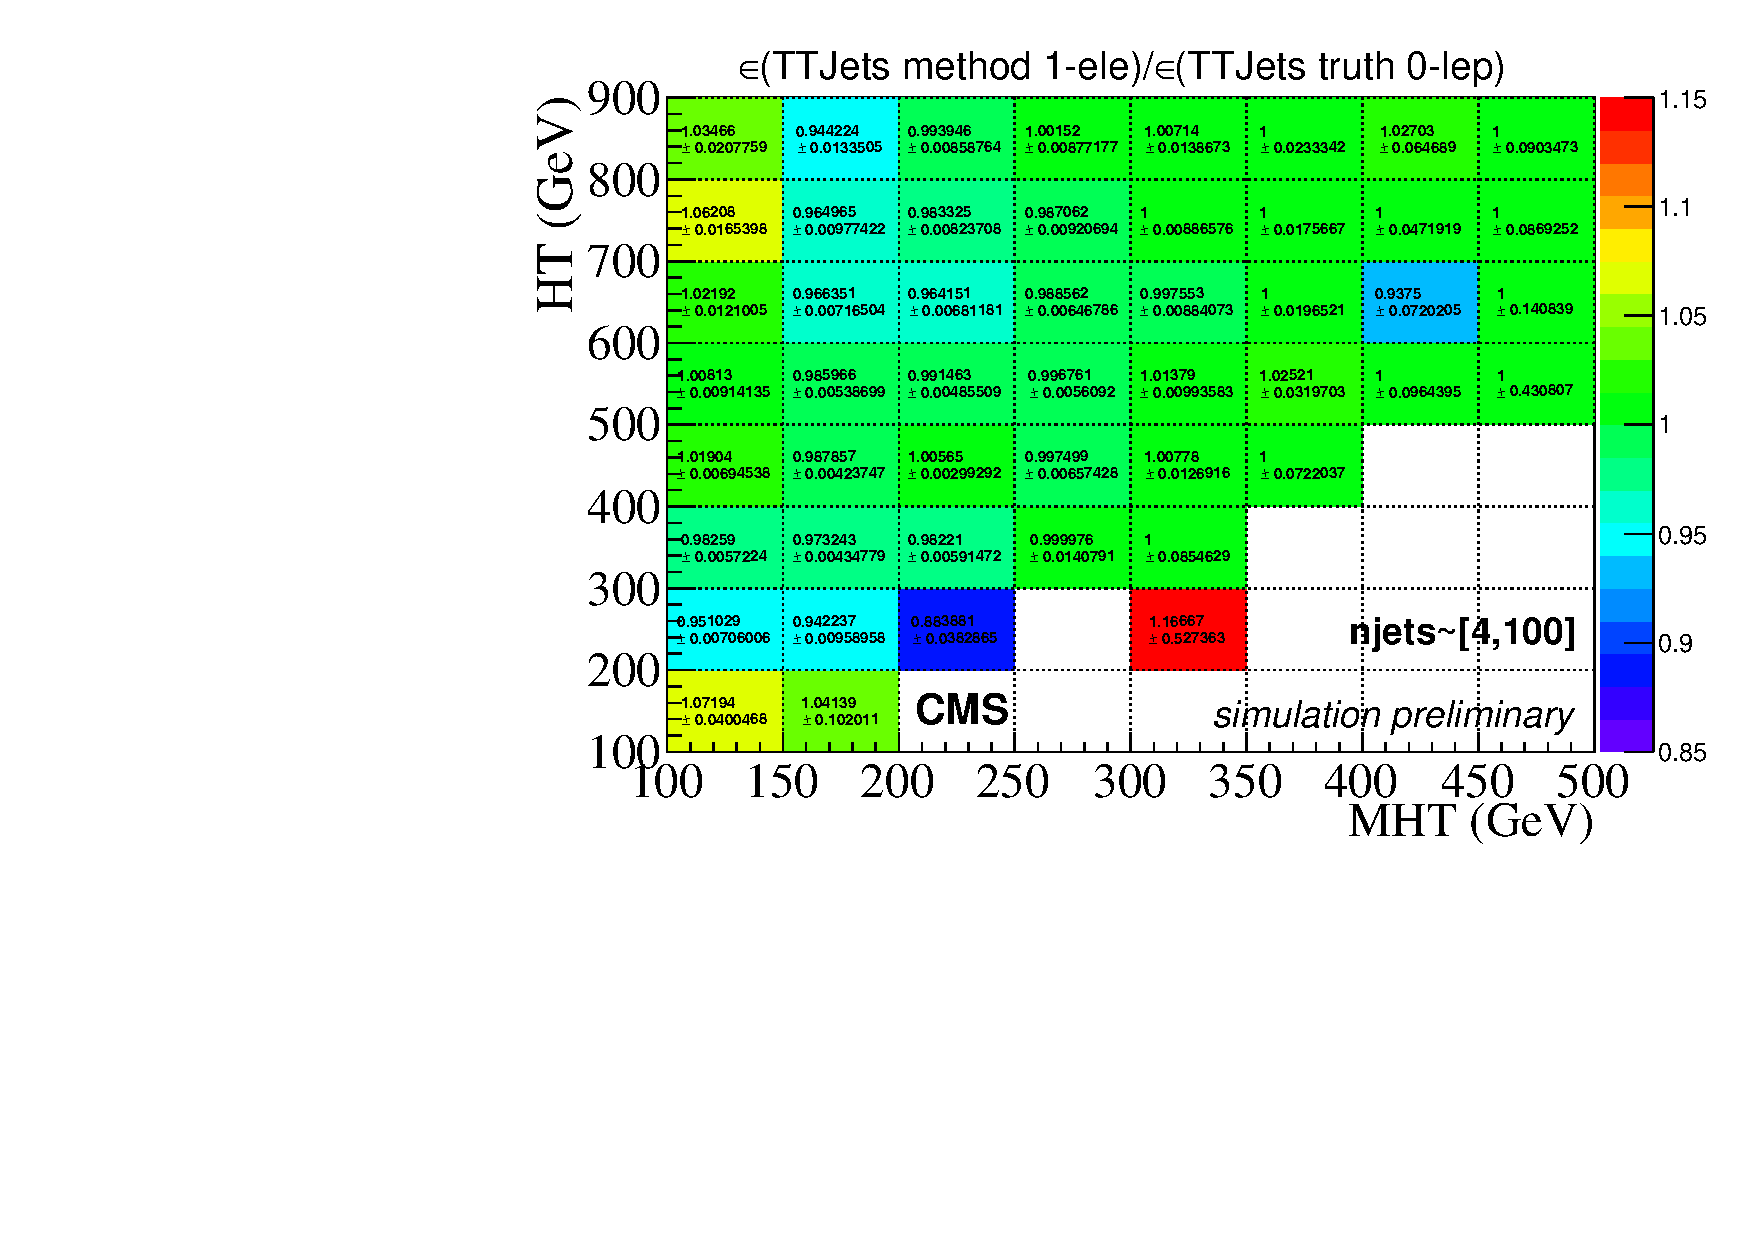
\includegraphics[width=0.95\linewidth]{figures/trigger/MonojetTrigger_EfficiencyRatioMC.pdf}
    \caption{
      The ratio of the monojet trigger efficiency for events passing the single
      electron reference trigger to the trigger efficiency for all
      events in a simulated $\ttbar$ sample, as a function of the offline $\Ht$
      and $\mht$. The ratio is consistent with 1 throughout the $\Ht-\mht$ plane.}
    \label{fig:2dMonoEffRatio}
  \end{center}
\end{figure}
\FloatBarrier
 \noindent
 The monojet trigger is a promising candidate for future analyses that search for evidence of SUSY in the low-$\Ht$ and low-$\mht$ regions, for which it was found that large nonexcluded SUSY cross sections could be manifest in the current data. 
 
\subsubsection{Multivariate efficiency }
\label{sec:mvatrigger}
It is possible for the trigger efficiency to vary as a complicated function of the observables in events. Often, a trigger decision involves a long chain of HLT (Chapter \ref{chap:cms} Section \ref{sec:Trigger}) modules, or filters, that can potentially induce unforeseen dependencies of the probability of firing the trigger on non-trivial correlations among the observables. One way to account for these correlations is to increase the dimensionality of the parametrization of the trigger efficiency estimation. For example, the jet multiplicity could be added as a third dimension to accompany the previously described $\Ht$ and $\mht$ parameterization if it were believed that $\njets$ were a determinant of the efficiency. However, adding additional dimensions requires the division of the event sample into a larger number of bins, which reduces the counts in each bin. This approach is ultimately plagued by the curse of dimensionality.

It is possible to reduce the dimensionality of the parametrization to just 1 dimension by constructing an appropriate single-valued function of the relevant observables. Such a function can be obtained through the use of a Bayesian neural network (NN) classifier, as previously demonstrated by Sezen Sekmen, Wee Don Teo, and Harrison Prosper in the context of b-tagging triggers \cite{bib:SezenTrigger}. 

As stated in Equation \ref{eq:mlp}, the output of such a classifier can be interpreted as
\begin{equation}
\text{NN} = P(\text{s}|\vec{\theta}) = \frac{p(\vec{\theta} | {\rm s})}{p(\vec{\theta} | {\rm s})+p(\vec{\theta} | {\rm b})},
\end{equation}
where $\vec{\theta}$ is a vector of observed quantities, also called the data, and s and b are, respectively, the true and false outcomes\textemdash in this case, the decision made by the trigger whether to fire. Since a NN is capable of training with a vector $\theta$ of arbitrary length, it is worth including any observable that may be relevant for the determination of the efficiency. To train the NN for the monojet trigger efficiency, the single electron reference sample is divided into events that fire the monojet trigger, which serve as the signal training events, and events that fail the monojet trigger, which serve as the background training events. There are several internal NN parameters, which govern aspects of the output such as the responsiveness of the output to small fluctuations in the data. These parameters are assigned gaussian prior probability densities that are broad distributions relative to the likelihood functions, which are highly corrugated. This results in posterior densities for the NN parameters that are dominated by the likelihoods. To obtain an uncertainty in the efficiency estimate, the posterior densities of the NN parameters are randomly sampled, and an ensemble of efficiency estimates are obtained. The mode of the envelope of this ensemble defines the central efficiency estimate, and the uncertainty band taken as the interval that is centered on the mode and contains 68\% of the estimated efficiency values. 

Figure \ref{fig:mvatrigger} shows the dependence of the monojet trigger efficiency on a few kinematic variables, both for the NN-derived efficiency and the efficiency computed in the traditional way. As values of the $\Ht$ are scanned over, the NN efficiency reveals a dependence on correlations between the $\Ht$ and $\mht$. Importantly, this manifests as the loss of efficiency for very high $\Ht$ around $\mht\approx200-300$ GeV.

\begin{figure}[tbp]
  \begin{center}
    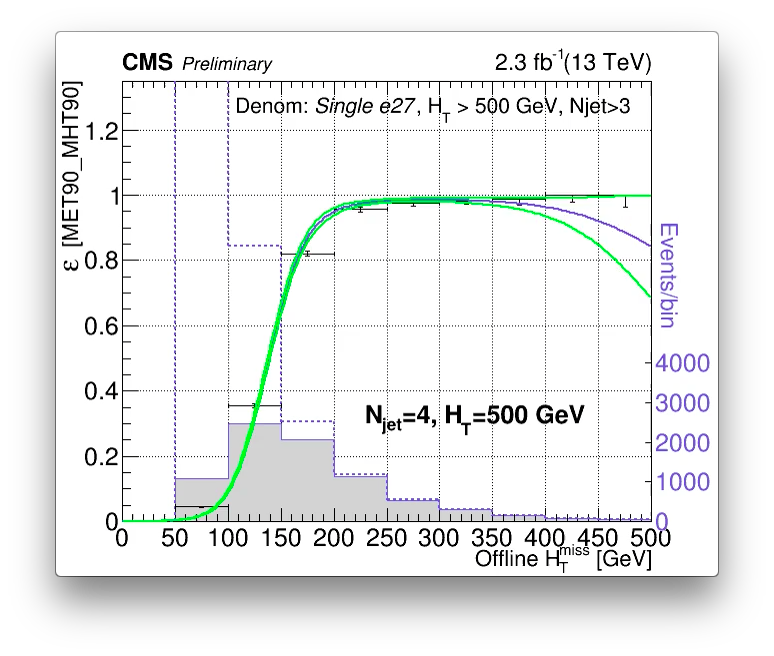
\includegraphics[width=0.49\linewidth]{figures/trigger/MonoTrigEff_Ht500.png}
    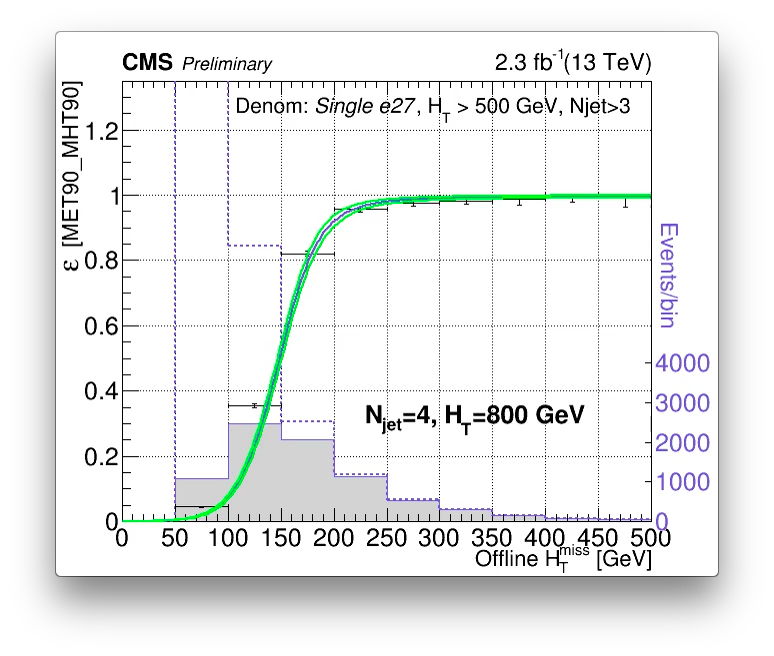
\includegraphics[width=0.49\linewidth]{figures/trigger/MonoTrigEff_Ht800.png}\\
        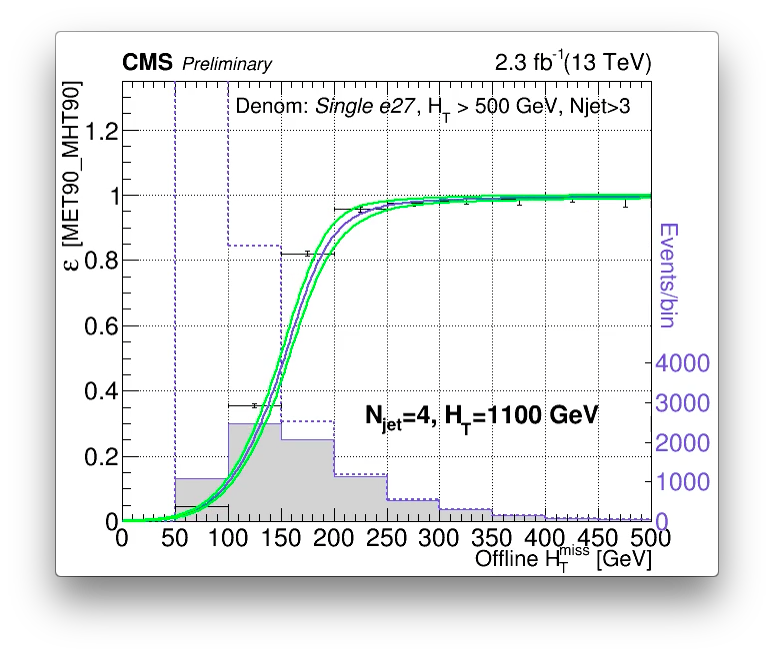
\includegraphics[width=0.49\linewidth]{figures/trigger/MonoTrigEff_Ht1100.png}
    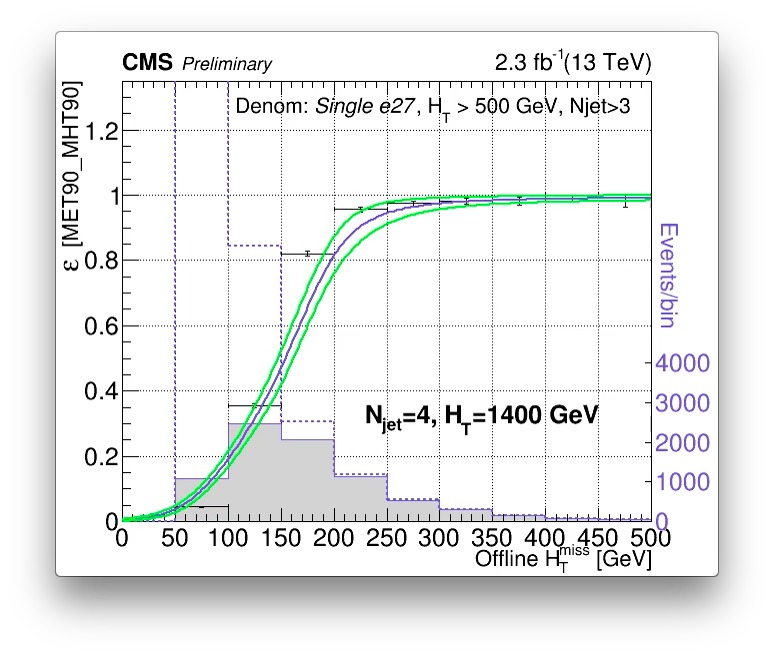
\includegraphics[width=0.49\linewidth]{figures/trigger/MonoTrigEff_Ht1400.png}\\
        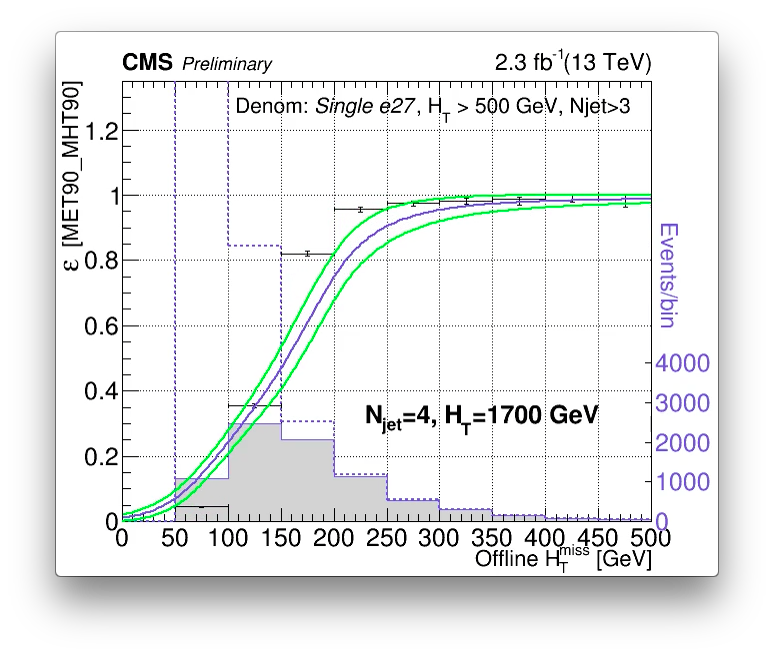
\includegraphics[width=0.49\linewidth]{figures/trigger/MonoTrigEff_Ht1700.png}
    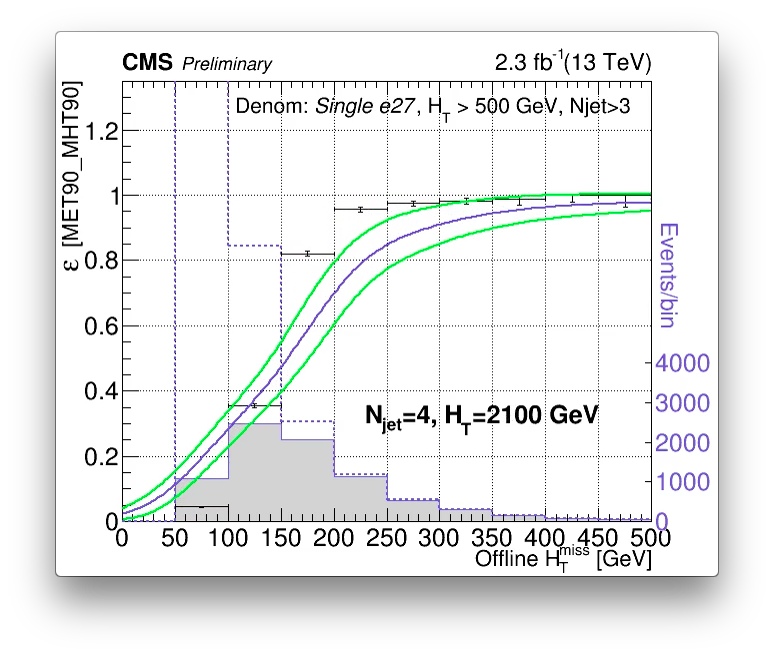
\includegraphics[width=0.49\linewidth]{figures/trigger/MonoTrigEff_Ht2100.png}
    \caption{The trigger efficiency as a function of the offline $\mht$ for the monojet trigger, measured the traditional way (histograms) and by the NN method (blue function), for $\njets=4$, with varying values of the $\Ht$. The green function lines show the 1-sigma uncertainty on the efficiency. }
    \label{fig:mvatrigger}
  \end{center}
\end{figure}
\FloatBarrier
\noindent
This method constitutes a robust model for the trigger that is particularly well-suited for analyses that consider events in regions of kinematic phase space in which the trigger efficiency is varying as a function of the observables.  Typically, analyses, attempt to avoid such regions, since traditional trigger efficiency estimation techniques can hide potentially detrimental effects in these regions, such as the efficiency loss at high $\Ht$ revealed in Fig. \ref{fig:mvatrigger}. Such kinematic regions include the low to moderate $\Ht$ and $\mht$ regions, which were identified as potentially signal rich.
